\documentclass[conference]{IEEEtran}
\IEEEoverridecommandlockouts

% --- Поддержка русского языка и кодировок ---
\usepackage[T2A]{fontenc}
\usepackage[utf8]{inputenc}
\usepackage[english,russian]{babel}

% --- Базовые математические пакеты IEEE ---
\usepackage{amsmath,amssymb,amsfonts}
\usepackage{cite}
\usepackage{textcomp}
\usepackage{xcolor}

% --- Графика и таблицы ---
\usepackage{graphicx}
\graphicspath{{fig/}}
\usepackage{booktabs}
\usepackage{array}
\usepackage{microtype}

% --- Ссылки и URL ---
\usepackage{url}
\def\UrlBreaks{\do\/\do-\do_}
\usepackage{hyperref}
\hypersetup{
    colorlinks=true,
    linkcolor=black,
    filecolor=black,
    urlcolor=blue,
    citecolor=black
}

% --- Переопределение названий окружений под русский язык IEEE ---
\addto\captionsrussian{%
  \renewcommand{\figurename}{Рис.}%
  \renewcommand{\tablename}{ТАБЛИЦА}%
  \renewcommand{\abstractname}{Аннотация}%
}


\begin{document}

\title{Сквозное аппаратно-программное моделирование тракта параллельного поиска сигналов GPS L1 с использованием Verilator}

\author{\IEEEauthorblockN{И.\,А.~Мартыненко}
\IEEEauthorblockA{\textit{Кафедра радиотехнических систем} \\
\textit{Национальный исследовательский университет «МЭИ»}\\
Москва, Россия \\
MartynenkoIA@mpei.ru, ORCID: 0009-0005-5176-0151}
}

\maketitle

\begin{abstract}
Разработка бортовых навигационных приемников для малых космических аппаратов (МКА) формата CubeSat требует применения алгоритмов параллельного поиска (PCPS) для преодоления высокой динамики доплеровского сдвига. Однако традиционное событийно-управляемое моделирование таких трактов сталкивается с вычислительным барьером при обработке длинных выборок сигнала. В данной работе предложена методология сквозной верификации тракта первичного поиска GPS L1, объединяющая синтезируемую RTL-модель на SystemVerilog и программное окружение на C++ в единый исполняемый файл с помощью компилятора Verilator. Использование статического планирования графа схемы и нативной интеграции C++ позволило реализовать адаптивный детектор Неймана--Пирсона с оценкой шума по выборке без накладных расходов на межъязыковое взаимодействие. Экспериментальные результаты на модели сигнала с отношением сигнал/шум $-20$~дБ подтвердили работоспособность комплекса: полное сканирование пространства «задержка--Доплер» в диапазоне $\pm50$~кГц (201 частотный срез) выполнено за один прогон симуляции.
\end{abstract}

\begin{IEEEkeywords}
GPS L1, первичный поиск, PCPS, критерий Неймана--Пирсона, Verilator, CubeSat, SystemVerilog, HW/SW Co-design, ASIC.
\end{IEEEkeywords}

\section{Введение}

Специфика функционирования малых космических аппаратов (МКА) формата CubeSat на низких околоземных орбитах (LEO) накладывает жёсткие ограничения на архитектуру бортовой аппаратуры спутниковой навигации. Высокая орбитальная скорость движения платформы сопровождается значительным доплеровским сдвигом несущей частоты принимаемых радиосигналов GPS L1 и его высокой динамикой. Это многократно расширяет область неопределённости в пространстве параметров <<задержка--Доплер>>, требуя применения алгоритмов параллельного поиска по кодовой фазе (Parallel Code Phase Search, PCPS) для обеспечения приемлемого времени <<холодного>> старта навигационного приёмника.

Реализация алгоритма PCPS на ПЛИС связана с непрерывной обработкой потока отсчётов с высокой частотой дискретизации и выполнением ресурсоёмких процедур согласованной фильтрации на базе быстрого преобразования Фурье. Традиционный маршрут проектирования таких трактов опирается на проприетарные САПР и событийно-управляемые симуляторы логического уровня. Однако проверка алгоритмов захвата на длинных сигнальных выборках физического эфира сталкивается с вычислительным барьером, обусловленным накладными расходами событийно-управляемой симуляции.

В данной работе предлагается рассмотреть решение этой проблемы переходом к методологии совместного аппаратно-программного моделирования с применением компилятора Verilator. Согласно исследованиям \cite{cornell, ieee_ble} такой подход обеспечивает качественно иной характер зависимости времени симуляции от объёма моделируемой схемы, что снижает время сквозной верификации при возрастании объёма модели.

Целью настоящей работы является разработка и экспериментальное исследование сквозного аппаратно-программного комплекса первичного поиска навигационных сигналов GPS L1 C/A. Предложенная методология объединяет синтезируемый RTL-тракт цифровой обработки сигналов и высокопроизводительный верификационный стенд на базе Verilator.

\section{Аппаратная архитектура тракта поиска}


\begin{figure*}[!t]
    \centering
    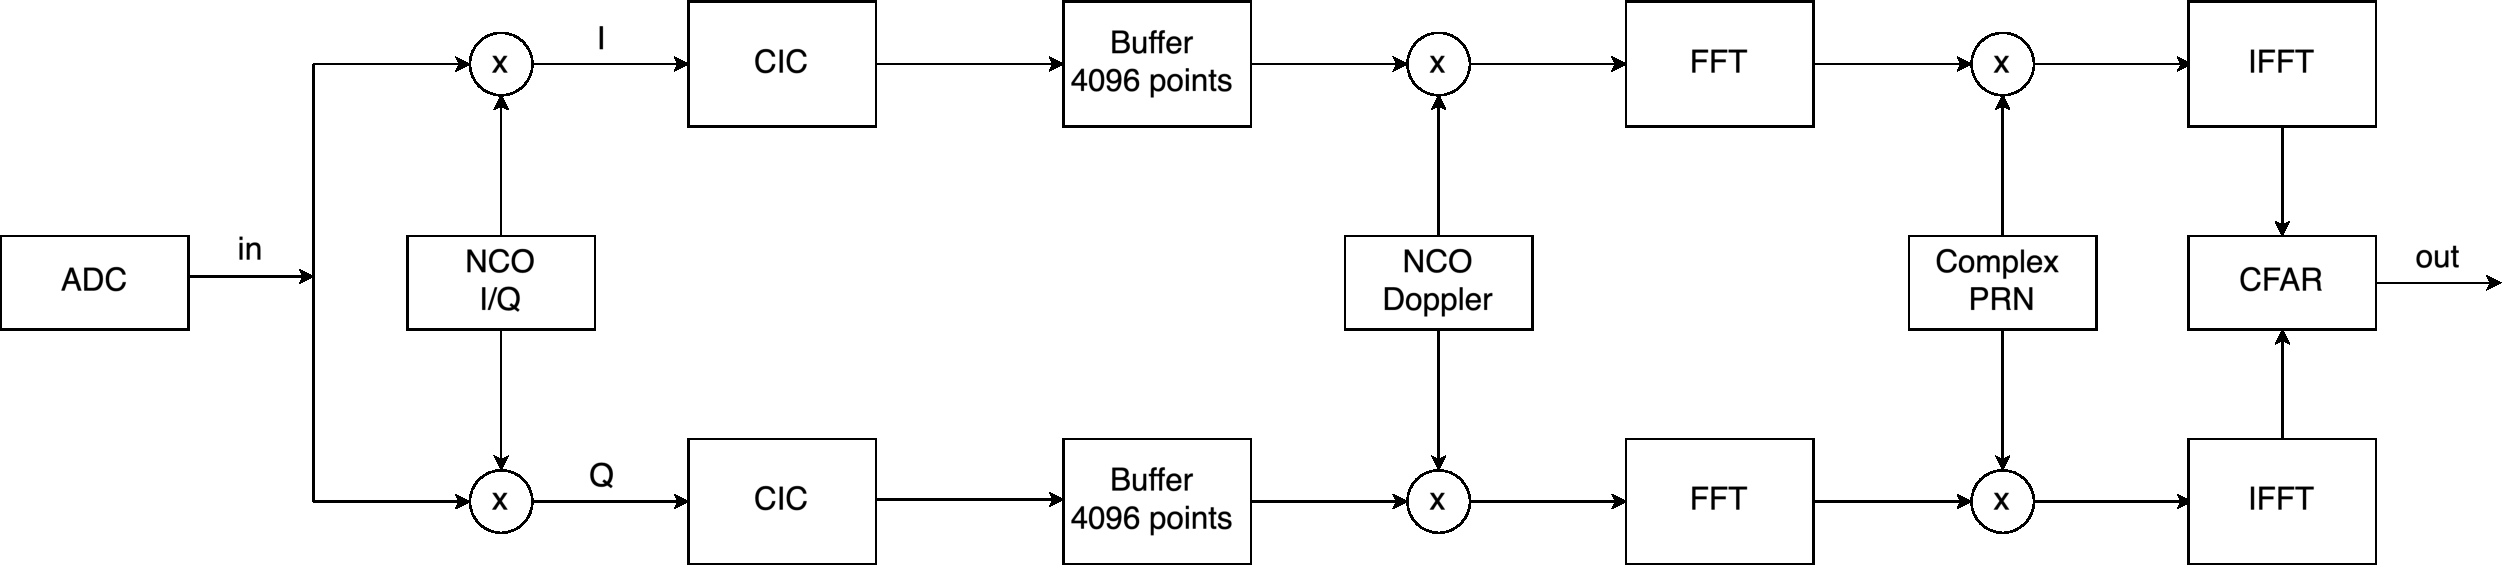
\includegraphics[width=0.9\textwidth]{coarse.pdf}
    \caption{Структурная схема тракта первичного поиска сигналов GPS L1}
    \label{fig:arch}
\end{figure*}

Вычислительный тракт параллельного поиска реализует согласованную фильтрацию входного радиосигнала. Его обобщенная структурная схема представлена на рис.~\ref{fig:arch}. На вход тракта от блока АЦП поступает цифровой поток промежуточной частоты $f_{\text{IF}} = 9{,}548$~МГц при частоте дискретизации $F_s = 38{,}192$~МГц.

\textbf{Квадратурный перенос на нулевую частоту.}
Входной оцифрованный сигнал поступает на блок квадратурного гетеродина (DDC), осуществляющий перенос спектра на нулевую промежуточную частоту путем умножения на отсчеты синусной и косинусной составляющих цифрового генератора:
\begin{equation}
    \begin{cases}
        I[n] = D_{\text{adc}}[n] \cdot \cos(\phi[n]), \\
        Q[n] = D_{\text{adc}}[n] \cdot \sin(\phi[n]).
    \end{cases}
\end{equation}
Поскольку в тракте применен 1-битный АЦП ($D_{\text{adc}}[n] \in \{-1, 1\}$), аппаратная реализация не требует использования многоразрядных умножителей, операция умножения сводится к инверсии знака табличного отсчета NCO в зависимости от текущего бита АЦП.

\textbf{Фильтрация и децимация.}
Сформированные квадратурные компоненты $I[n]$ и $Q[n]$ содержат высокочастотные составляющие спектра на удвоенной промежуточной частоте. Для их подавления и снижения вычислительной нагрузки на последующие блоки тракта применены каскадные интегрально-гребенчатые фильтры (CIC). Модуль осуществляет децимацию входного потока с коэффициентом $R = 10$, понижая исходную частоту дискретизации $F_s = 38{,}192$~МГц до темпа обработки $F_{\text{dec}} = 3{,}8192$~МГц. Выбор CIC-архитектуры обусловлен отсутствием умножителей в ее структуре, что минимизирует площадь кристалла и снижает энергопотребление тракта.

\textbf{Буферизация и дополнение нулями.}
С выхода CIC-фильтров отсчеты квадратурных составляющих поступают в буфер согласования базы. За период повторения дальномерного C/A-кода GPS ($T_{\text{coh}} = 1$~мс) на децимированной частоте $F_{\text{dec}} = 3{,}8192$~МГц накапливается массив из 3819 комплексных отсчетов с точностью до целой части. Для применения radix-2 алгоритма БПФ массив дополняется нулями (zero-padding) до размерности N=4096 отсчётом, при этом уровень наложения циклической корреляции остаётся допустимым и не влияет на положение главного корреляционного пика.

\textbf{Компенсация доплеровского смещения.}
Для устранения частотной неопределенности, вызванной движением космического аппарата, формируется сетка доплеровских гипотез с постоянным шагом $\Delta f_d = 500$~Гц. Перед процедурой спектрального согласованного поиска накопленный в буфере комплексный вектор отсчетов последовательно перемножается на квадратурные составляющие вторичного гетеродина (NCO Doppler), настроенного на соответствующее смещение частоты:
\begin{equation}
    f_{\text{dop}}^{(m)} = m \cdot \Delta f_d, \quad m \in [-M, M],
\end{equation}
где $m$ — номер текущей проверяемой гипотезы. Скомпенсированный во временной области сигнал передается на блок согласованной фильтрации.

\textbf{Согласованная фильтрация и спектральный анализ.}
Для каждой проверенной гипотезы по доплеровскому смещению выполняется процедура быстрого поиска на основе теоремы о свертке. Временной сигнал преобразуется в частотную область с помощью быстрого преобразования Фурье (БПФ), после чего его спектр поэлементно умножается на комплексно сопряженный опорный спектр локального C/A-кода спутника:
\begin{equation}
    Y[k] = X[k] \cdot S^*[k] = (X_I S_I + X_Q S_Q) + j(X_Q S_I - X_I S_Q).
\end{equation}
Затем с помощью обратного преобразования Фурье (ОБПФ) данные возвращаются во временную область, образуя отсчеты автокорреляционной функции. Детальные аппаратные особенности этого конвейера, а также результирующие поверхности отклика будут подробно рассмотрены в следующих разделах работы.

\textbf{Адаптивное пороговое обнаружение.}
Завершающим этапом тракта является блок пороговой обработки по критерию Неймана--Пирсона. На основе квадратов квадратурных составляющих $I^2[k] + Q^2[k]$ модуль формирует двумерную матрицу автокорреляционных откликов в пространстве «задержка--доплеровский сдвиг». Для квадратичного детектора при гауссовом шуме порог, обеспечивающий заданную вероятность ложной тревоги, определяется аналитически:
\begin{equation}
T = -\hat{\sigma}^2 \ln P_{\text{fa}}.
\end{equation}
где вероятность ложной тревоги $P_{\text{fa}} = 10 ^{-5}$.

%! TeX root = ../main.tex
\section{Методология верификации и обоснование выбора Verilator}

Тракт первичного поиска навигационных сигналов сочетает потоковую цифровую фильтрацию высокой интенсивности и алгоритмы статистической обработки откликов. Аппаратный блок на базе SystemVerilog реализует квадратурный перенос, децимацию и циклическую свёртку методом PCPS. Принятие решений об обнаружении и пороговая обработка по критерию Неймана--Пирсона вынесены в программную часть, требующую операций с плавающей точкой.

Интеграция RTL-тракта с программным окружением в классических САПР (ModelSim, Questa, Vivado XSIM) требует использования интерфейса DPI-C, что влечет за собой накладные расходы на согласование типов данных и организацию вызовов между ядром симулятора и внешним кодом.

В качестве альтернативы в работе применён свободно распространяемый компилятор Verilator с открытым исходным кодом, что снимает организационные и финансовые ограничения на развёртывание среды верификации. Verilator осуществляет статическое планирование графа схемы, компилируя логику в детерминированную последовательность инструкций C++ с использованием 2-state логики.

Ключевым преимуществом выбранной методологии является нативная интеграция с языком C++. Топ-модуль алгоритма PCPS инкапсулируется в C++ объект, регистры и порты которого доступны как поля структуры в едином адресном пространстве процесса. Благодаря этому исключается промежуточная буферизация, а любые сторонние библиотеки подключаются к симуляции напрямую.

\section{Результаты моделирования и экспериментальные исследования}

Для подтверждения работоспособности предложенного аппаратно-программного комплекса был проведен ряд симуляций с использованием модели смеси сигнала GPS L1 C/A и шума с отношением сигнал/шум \(-25\)~дБ и динамикой доплеровского сдвига \(-80\)~Гц/с при начальном значении Доплеровского сдвига равным $521$~Гц. С учетом высокой орбитальной динамики МКА на низких орбитах, диапазон сканирования был установлен от \(-50\) до \(+50\)~кГц с шагом 500~Гц, что сформировало 201 частотный срез.

На рис.~\ref{fig:spectra} представлены спектры сигнала на промежуточной частоте. Спектр после прямого БПФ (рис.~\ref{fig:spectra}, слева) имеет равномерную широкополосную структуру, типичную для шумового сигнала на промежуточной частоте. После перемножения спектра сигнала на комплексно-сопряженный спектр опорного кода Голда (рис.~\ref{fig:spectra}, справа) наблюдается характерное изменение формы огибающей, обусловленное амплитудно-частотным спектром дальномерной псевдослучайной последовательности (ПСП). Ширина главного лепестка соответствует стандартной полосе C/A-кода (\(\pm 1{,}023\)~МГц)

\begin{figure}[htbp]
    \centering
    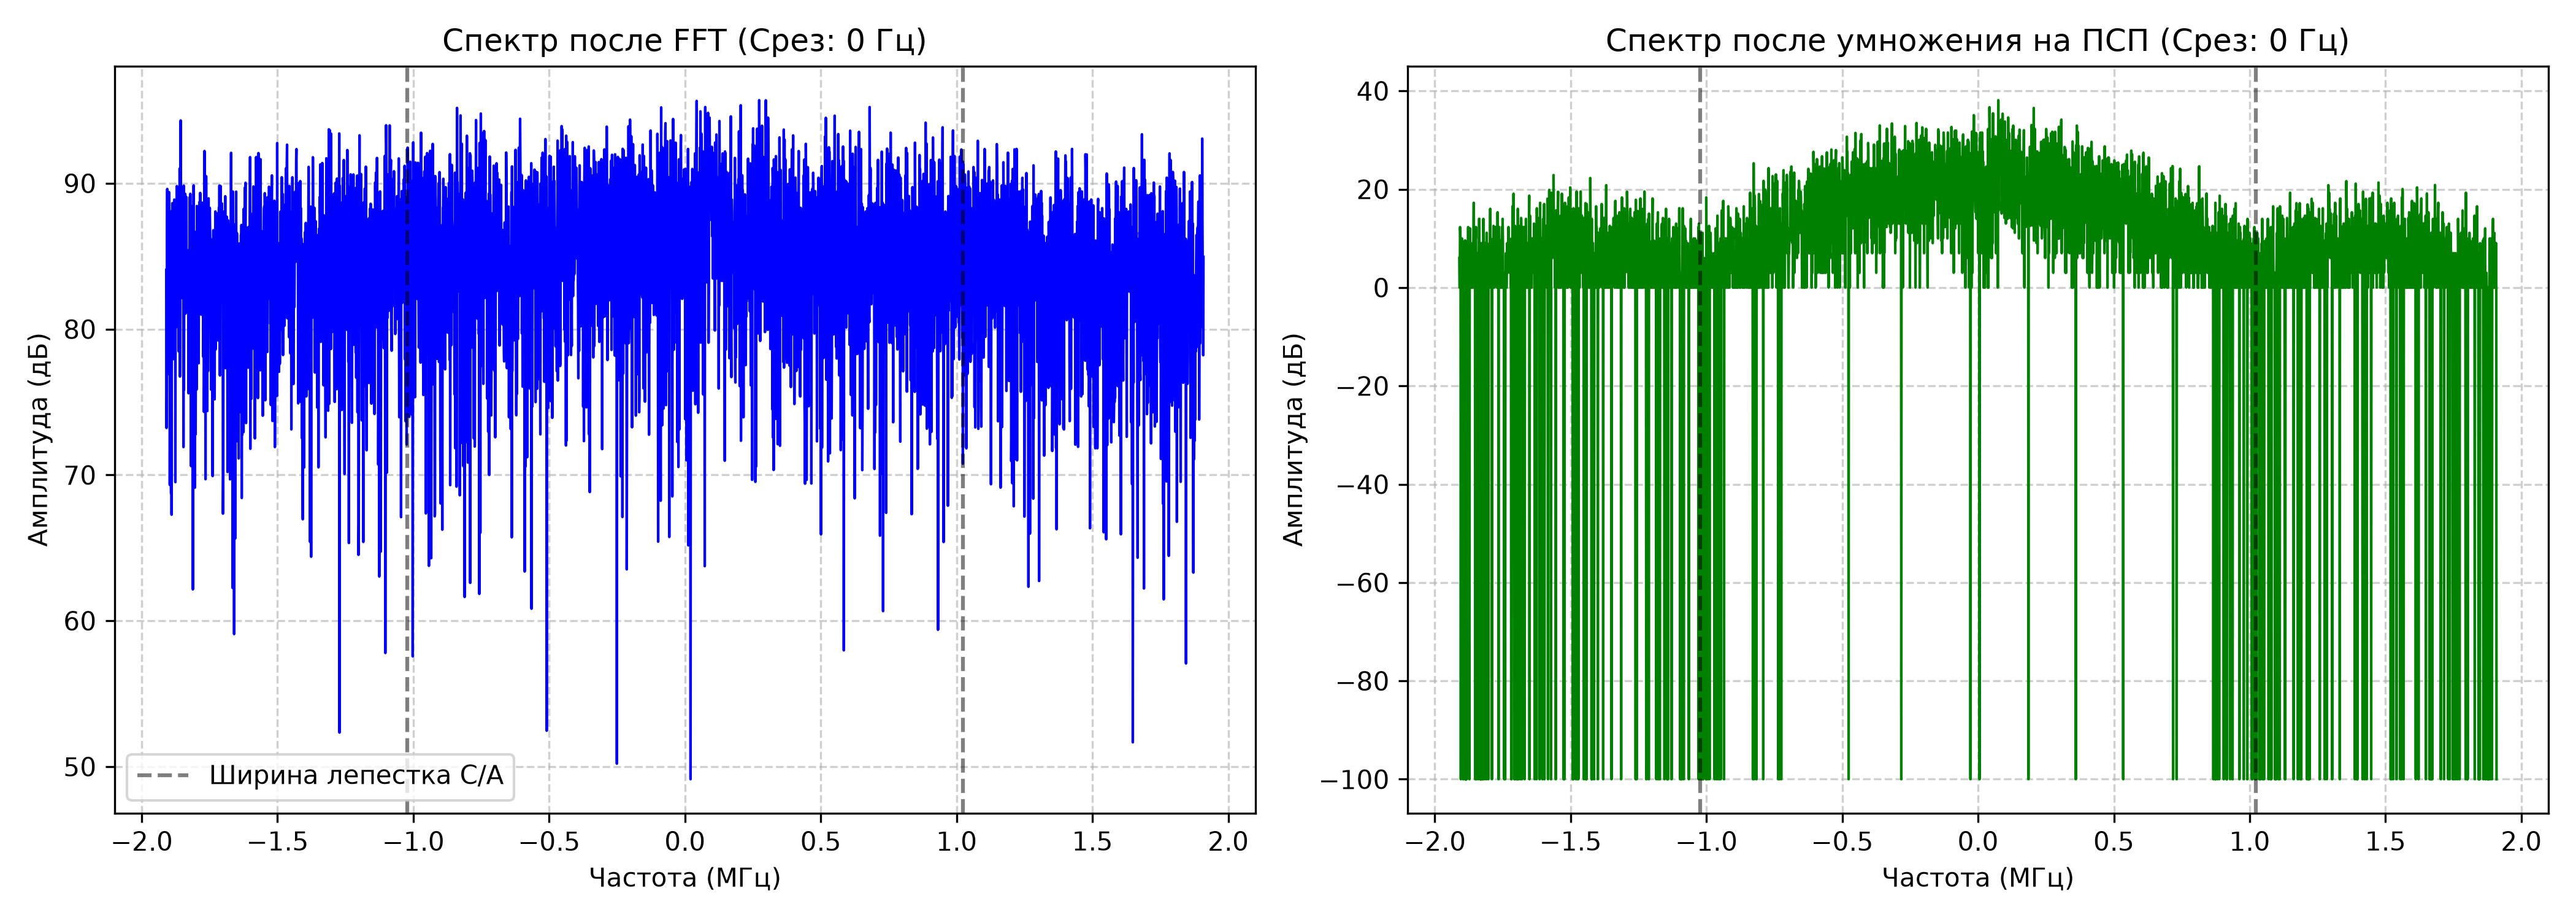
\includegraphics[width=\linewidth]{fig/fig1_spectra.png}
    \caption{Спектры сигнала после прямого БПФ (слева) и после перемножения на сопряженный спектр опорной ПСП (справа)}
    \label{fig:spectra}
\end{figure}

На рис.~\ref{fig:corr_slice} показан одномерный срез корреляционной функции по задержке кода при оптимальном доплеровском сдвиге 500~Гц. На фоне шумовой дорожки отчетливо выделяется узкий корреляционный пик, мощность которого на несколько порядков превышает уровень шума. Это свидетельствует о корректной работе конвейера согласованной фильтрации и высокой точности захвата по кодовой фазе.

\begin{figure}[htbp]
    \centering
    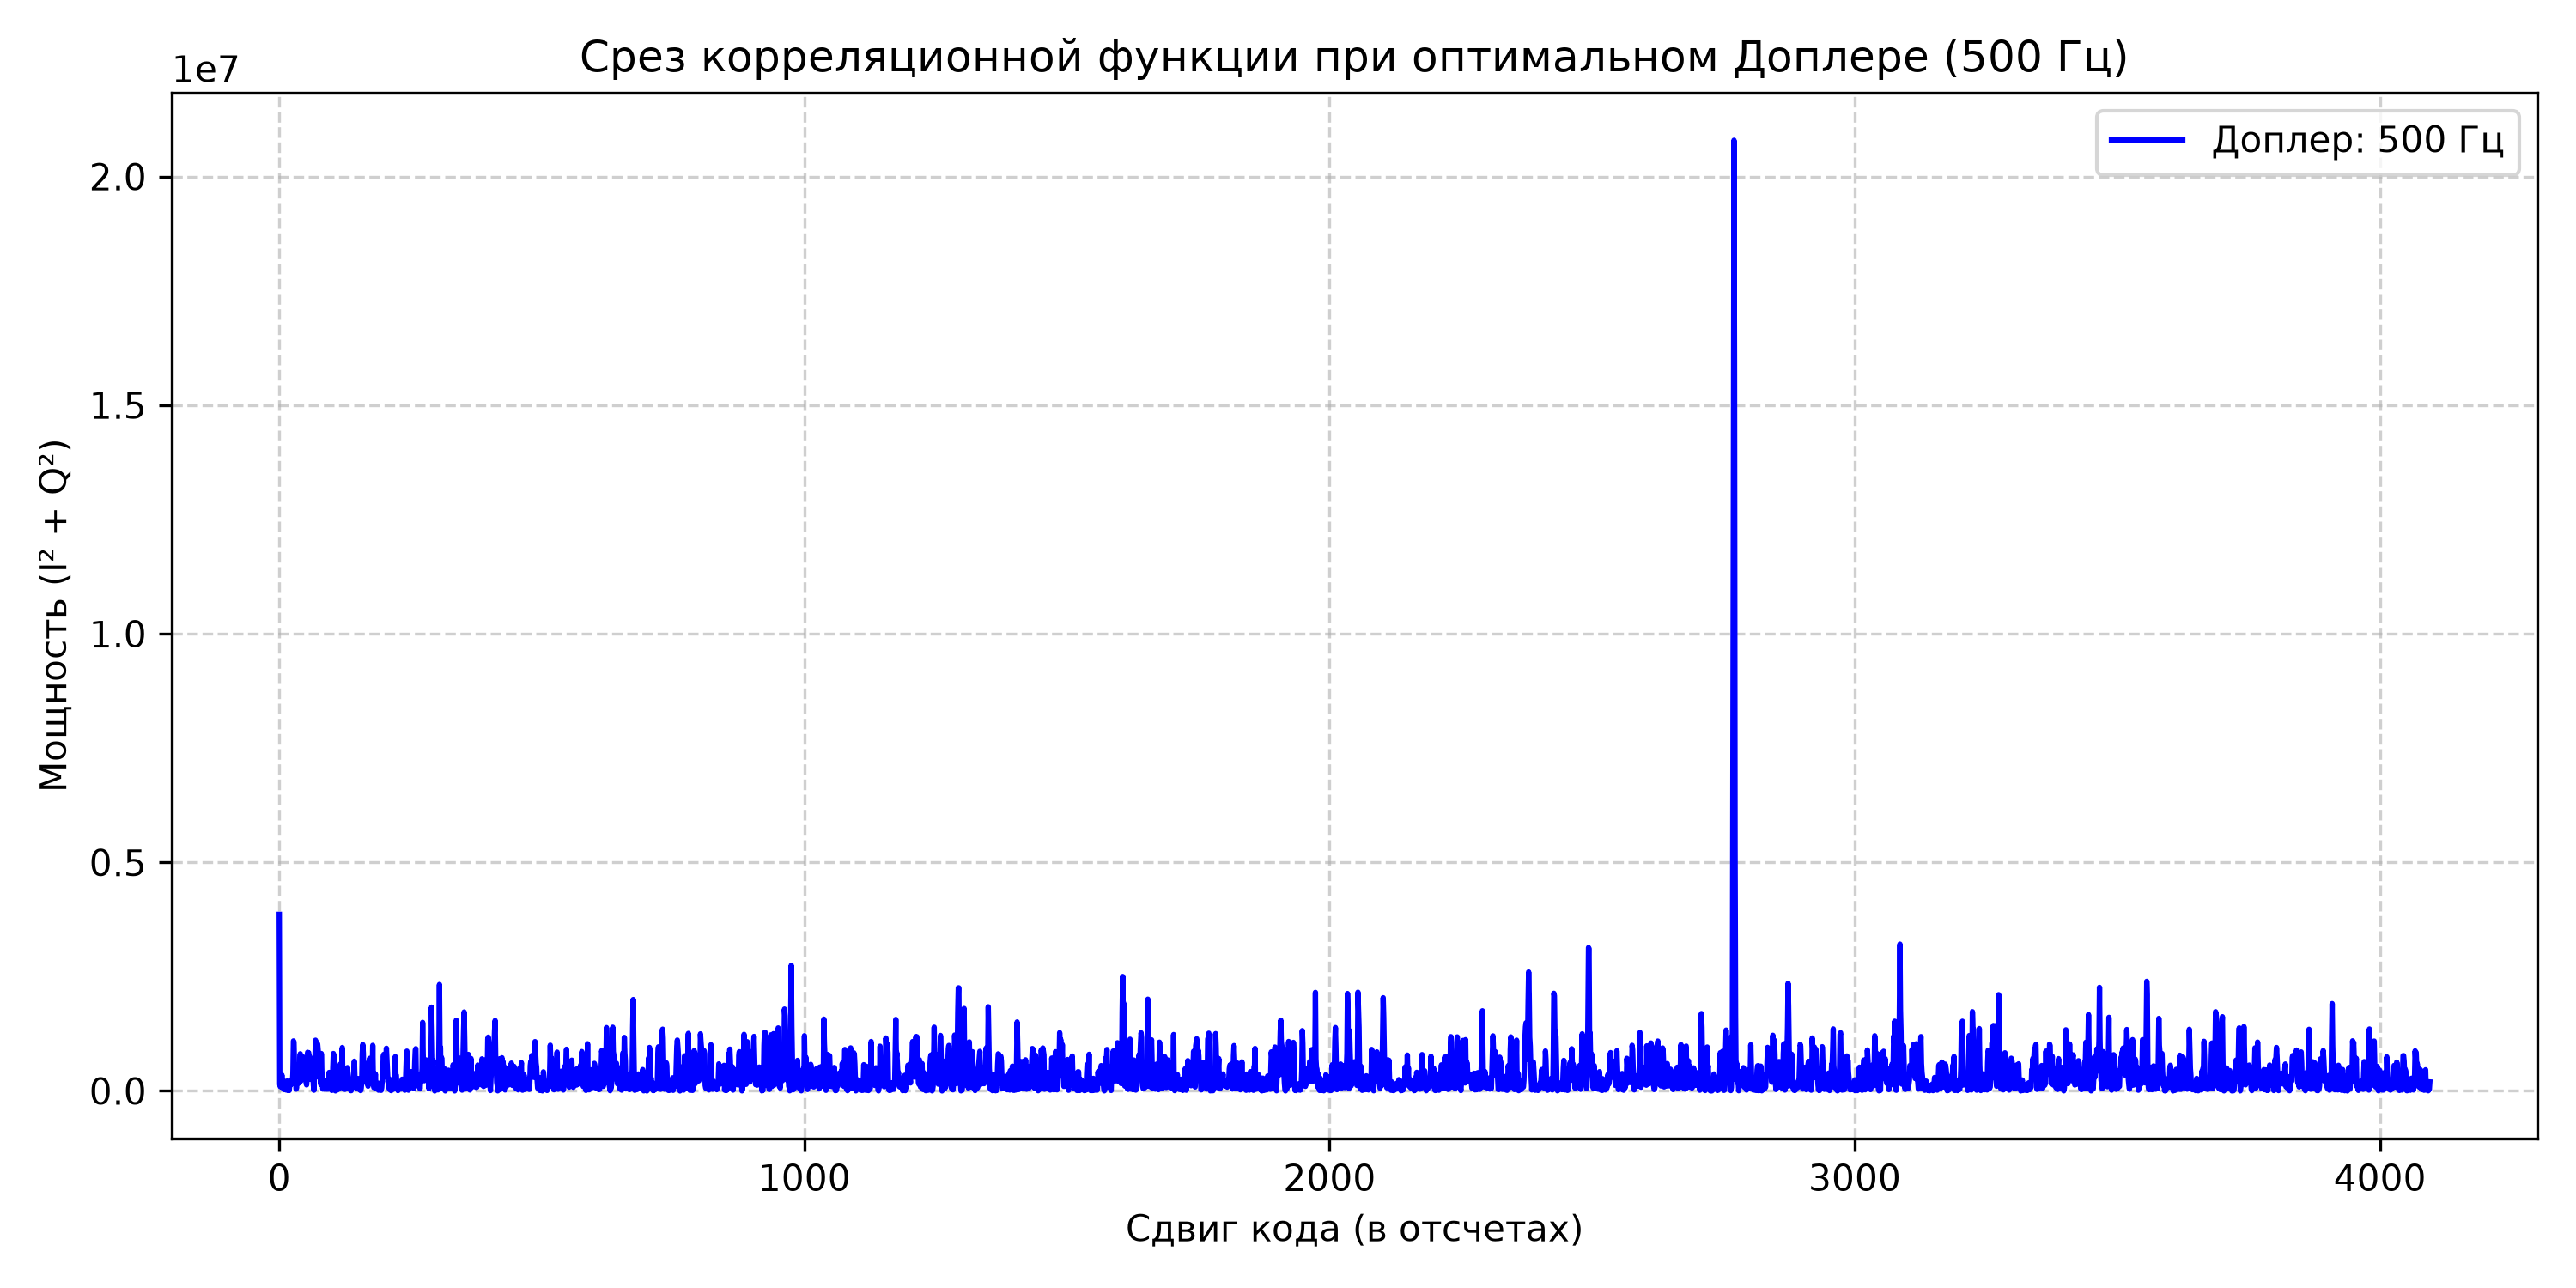
\includegraphics[width=\linewidth]{fig/fig2_doppler_slice.png}
    \caption{Срез корреляционной функции по кодовой задержке в оптимальном частотном канале ($f_d = +500$~Гц)}
    \label{fig:corr_slice}
\end{figure}

На рис.~\ref{fig:doppler_curve} приведена зависимость величины максимального корреляционного пика от проверяемой доплеровской частоты для всего диапазона \(\pm 50\)~кГц. На фоне равномерных шумовых выбросов амплитуда отклика резко возрастает только в узкой окрестности истинного значения (500~Гц), образуя ярко выраженный глобальный максимум.

\begin{figure}[htbp]
    \centering
    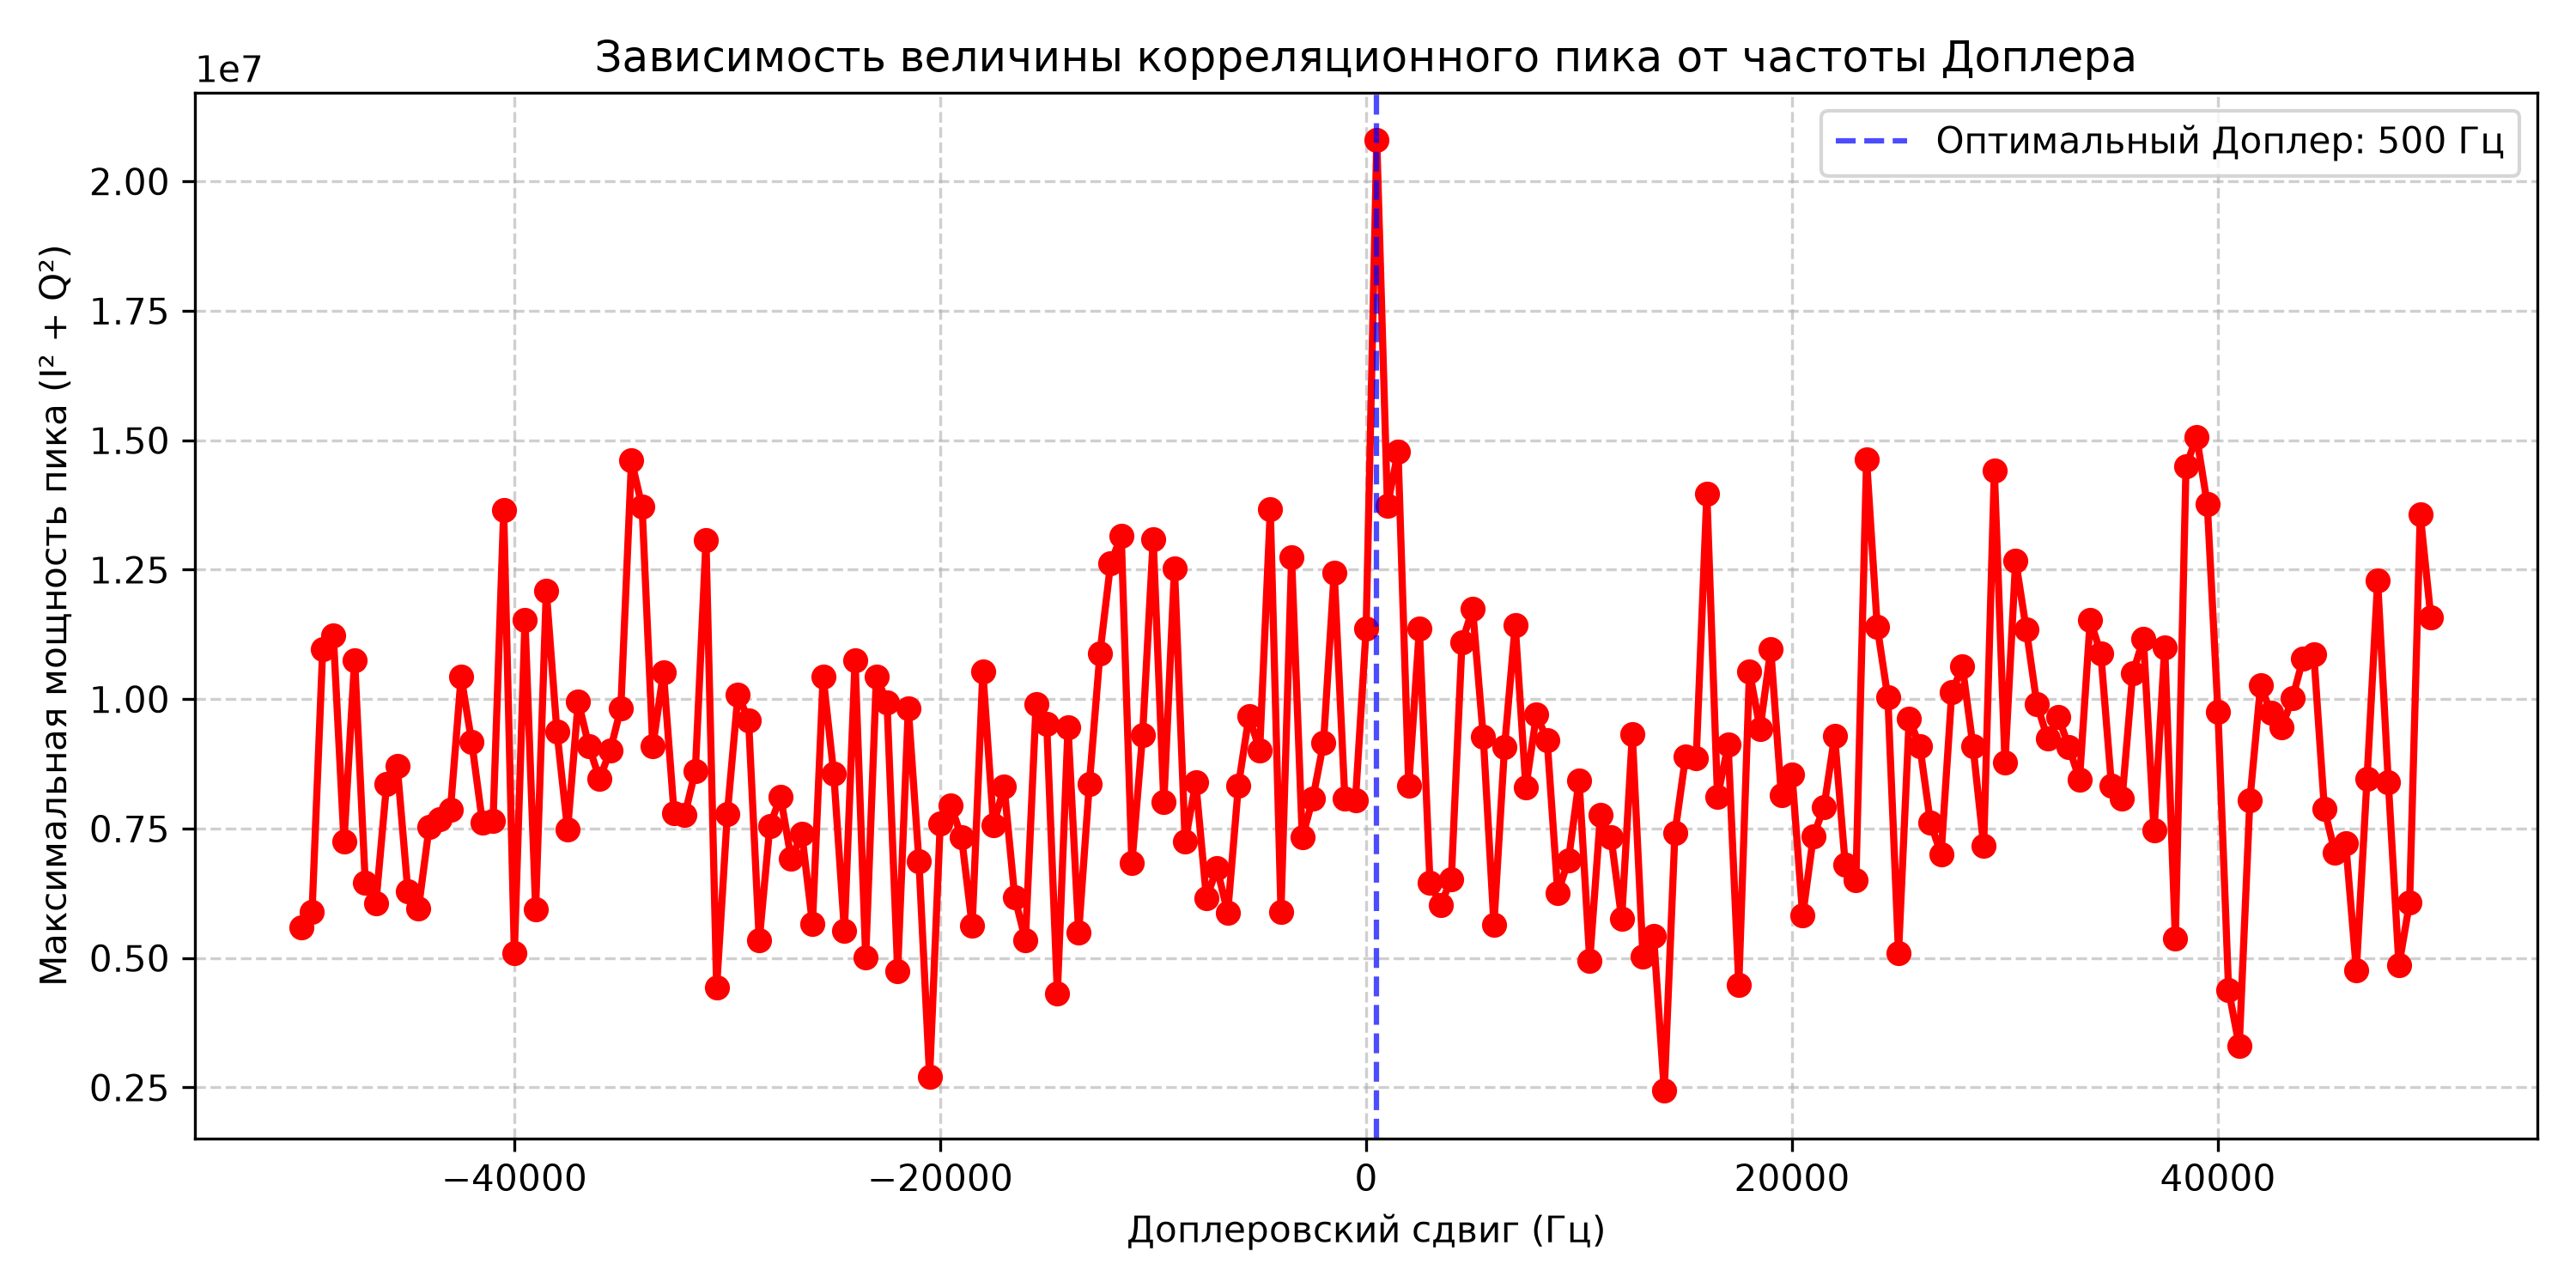
\includegraphics[width=\linewidth]{fig/fig4_peak_vs_doppler.png}
    \caption{Зависимость амплитуды корреляционного максимума от сдвига доплеровской частоты}
    \label{fig:doppler_curve}
\end{figure}



\section{Анализ производительности верификационного стенда}

Оценка вычислительной эффективности предложенного подхода проводилась при моделировании полного цикла работы навигационного приемника. Исходный массив оцифрованного сигнала имеет длительность 8 секунд, что необходимо для последующей работы канала слежения. Однако блок первичного поиска анализирует только фрагмент длительностью 1 мс, накапливая 4096 отсчетов после децимации. Поскольку алгоритм PCPS проверяет каждую из 201 доплеровской гипотезы независимо, симулятору требуется выполнить полный цикл конвейерной обработки (БПФ, перемножение и ОБПФ) для каждого среза. В результате полный цикл симуляции блока поиска потребовал непрерывного расчета \(11{,}87 \cdot 10^6\) тактов тактовой частоты схемы. После успешного обнаружения сигнала блок поиска отключается, а управление передается каналу слежения.

Ключевые параметры производительности среды на базе Verilator для этапа обнаружения приведены в табл.~\ref{tab:perf}. Пропускная способность симуляции достигла \(0{,}150\)~млн тактов в секунду, а общее время выполнения процесса составило около 80 секунд. 

Столь значительное время выполнения обусловлено высокой вычислительной сложностью алгоритма PCPS: для обработки всего одной миллисекунды сигнала требуется выполнить 201 независимый цикл согласованной фильтрации (каждый включает прямое БПФ, комплексное перемножение, обратное БПФ и квадратичное детектирование). Суммарно симулятору необходимо рассчитать более 400 преобразований Фурье размерностью 4096 точек, что эквивалентно \(11{,}87 \cdot 10^6\) тактов работы синхронного конвейера. При этом в отличие от классических событийно-управляемых симуляторов (Vivado XSIM, ModelSim), где на каждом такте формируются миллионы событий переключения триггеров и требуется их последовательная обработка через очередь планировщика, архитектура Verilator выполняет модель как единый нативный C++ процесс. 

Полученный показатель времени симуляции подтверждает пригодность данного подхода для практической верификации. Полный перебор 201 частотного среза для 1 мс выборки занимает менее полутора минут машинного времени. Это делает возможной итеративную отладку алгоритмов ЦОС, тогда как аналогичный тест в классических САПР требует значительно большего времени и вычислительных ресурсов.


\begin{table}[htbp]
\caption{Coarse Acquisition Performance}
\begin{center}
\begin{tabular}{|l|c|}
\hline
\textbf{Metric} & \textbf{Value} \\
\hline
Doppler bins & 201 \\
\hline
Simulated input-clock cycles & 11867040 \\
\hline
Acquisition time & 79.227 s \\
\hline
Total process time & 80.637 s \\
\hline
Simulation throughput & 0.150 Mcycles/s \\
\hline
Equivalent input time at 3.819 Msamples/s & 3.107 s \\
\hline
Speedup vs. input real time & 0.039 \\
\hline
\end{tabular}
\label{tab:perf}
\end{center}
\end{table}

\section{Заключение}
В работе предложена и экспериментально подтверждена методология сквозного аппаратно-программного моделирования тракта первичного поиска сигналов GPS L1 на базе компилятора Verilator. Разработанный комплекс объединяет синтезируемое RTL-описание алгоритма PCPS на SystemVerilog и программное окружение на C++.

Экспериментальные результаты на модели сигнала с отношением сигнал/шум \(-20\)~дБ подтвердили работоспособность верификационного стенда. Полное сканирование пространства параметров <<задержка--Доплер>> в диапазоне \(\pm50\)~кГц выполнено в рамках одного запуска симуляции. На сформированной двумерной поверхности отклика зафиксирован глобальный корреляционный пик, мощность которого на несколько порядков превышает уровень шума, что обеспечивает надежный захват сигнала при высокой динамике платформы.

Предложенный подход полностью снимает зависимость от проприетарных САПР на этапе верификации и ориентирован на последующую интеграцию разработанного тракта системы на кристалле (СнК) в составе бортовой аппаратуры малых космических аппаратов.


\begin{thebibliography}{99}

\bibitem{kaplan} Kaplan~E.~D., Hegarty~C.~J. Understanding GPS: Principles and Applications. --- 2nd ed. --- Norwood: Artech House, 2006. --- 703~p.

\bibitem{tsui} Tsui~J.~B.~Y. Fundamentals of Global Positioning System Receivers: A Software Approach. --- 2nd ed. --- New York: John Wiley \& Sons, 2005. --- 352~p.

\bibitem{borre} A Software-Defined GPS and Galileo Receiver: A Single-Frequency Approach / K.~Borre, D.~M.~Akos, N.~Bertelsen et al. --- Boston: Birkh{\"a}user, 2007. --- 176~p.

\bibitem{verilator} Snyder~W. Verilator: Fast, free, open-source SystemVerilog simulator // Veripool. --- 2024. --- URL: https://www.veripool.org/verilator/.

\bibitem{openlane} OpenLane: Open-Source ASIC Implementation Flow // Efabless Corporation. --- 2024. --- URL: https://github.com/The-OpenROAD-Project/OpenLane.

\bibitem{cornell} Rhod~E., Ghavami~B., Fang~Z., Shannon~L. A Cycle-Accurate Soft Error Vulnerability Analysis Framework for FPGA-based Designs // arXiv preprint arXiv:2303.12269. --- 2023. --- P.~1--10.

\bibitem{ieee_ble} Ham~E., Jeon~Y., Lim~J., Kim~J.~H. Verilator-based Fast Verification Methodology for BLE MAC Hardware // 2023 International Conference on Electronics, Information, and Communication (ICEIC). --- Singapore: IEEE, 2023. --- P.~1--5.

\end{thebibliography}


\end{document}
